\documentclass[a4paper,10pt]{report}
\usepackage[utf8]{inputenc}
\usepackage{graphicx}
\usepackage{subcaption}
\usepackage{wrapfig}

\newcommand{\comments}[1]{}

% Title Page
\title{Implémentation d'article de recherche \\ 
Removing Camera Shake via Weighted Fourier Burst Accumulation}
\author{Sofiane Horache, Roman Fenioux}
\date{April 2017}


\begin{document}
\maketitle


% pour éviter d'avoir la numérotation 0.1 0.2 etc avant les sections
\setcounter{secnumdepth}{0}

% 1st page, résumé de l'article
\section{Introduction}
\paragraph{}
Ce projet est une implémentation de l'article Removing Camera Shake via Weighted Fourier Burst Accumulation
proposé par Mauricio Delbracio et Guillermo Sapiro. \\


\paragraph{}
Le problème adressé ici est le flou de bougé, présent notamment dans les photographies 
amateur prises à la main dans des environnements mal éclairés. Pour avoir une photographie 
suffisament exposée il est souvent necessaire d'augmenter le temps d'exposition lorsqu'on 
ne peut ou ne veut pas agir sur l'ouverture ou la sensibilité de l'appareil. Mais si la 
position ou l'orientation de l'appareil change durant l'acquisition, on voit apparaître du flou dans la direction
du mouvement. 

\section{Approche de l'article}
\paragraph{}
Le mouvement de l'appareil durant la prise de vue est modélisé par une convolution de l'image
par un noyau de flou. la direction du mouvement est aléatoire d'une image à l'autre et on veut donc 
récupérer l'information que contient chaque image pour obtenir une image nette. L'approche utilisée 
ici consiste à prendre une rafale d'images au lieu d'une seule, puis à les combiner pour éliminer ce 
flou. Cette technique permet même de débruiter l'image. 
\paragraph{}
Pour une séquence de M images on a donc :
\[
  v_{i} = u_{i} \ast k_{i} + n{i}
\]
\paragraph{}
Pour ce faire l'article propose de calculer une moyenne pondérée de leurs transformées 
de Fourier pour éviter d'avoir à faire une estimation explicite du noyau de flou.
\[
  u_{p}(x) = \mathcal{F}^{-1}\left(\sum_{i=1}^M w_{i}(\zeta)\cdot \hat{v_{i}}(\zeta)\right)(x)
\]
\[
  w_{i}(\zeta) = \frac{|\hat{v_{i}}(\zeta)|^p}{\sum_{j=1}^M |\hat{v_{j}}(\zeta)|^p}
\]

\paragraph{}
Le parametre \(p\) est un entier qui contrôle la manière dont sont agrégés les résultats. Si \(p = 0\) la somme 
se ramène à une moyenne des transformées de Fourier des différentes images. Lorsque \(p \rightarrow \infty \) 
cela revient à prendre pour chaque fréquence la maximale qu'elle atteint dans une des images. 

\section{Notre implémentation }
\paragraph{}
Nous avons travaillé en C++ avec la librairie OpenCV.
\paragraph{}
Nous avons d'abord implémenté la méthode de l'article sur des images supposées bien recalées, puis
nous avons implémenté l'algorithme ORSA pour le recalage des images. 
Nous n'avons pas implémenté la détection des homographies dégénérées.
\\\\
Rappeler formules ORSA

\section{Nos résultats}

\subsection{Images déjà recalées}
Nous avons d'abord testé la méthode sur des images déjà recalées que nous avons crées
nous même en convoluant une image avec différents noyaux de flous correspondant pour simuler 
le mouvement de l'appareil. Dans la figure~\ref{fig:arctriomphe}
(page~\pageref{fig:arctriomphe}) on peut comparer le résultat obtenu à
l'image originale utilisée et à la meilleure des images floues.

\begin{figure}[h]
 
\begin{subfigure}{0.24\textwidth}
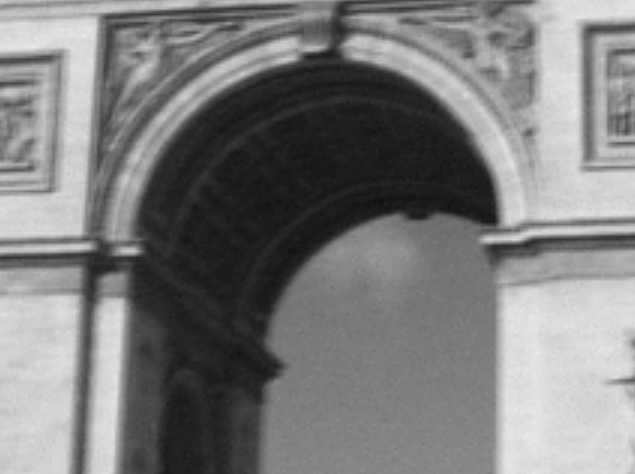
\includegraphics[width=0.9\linewidth]{ressource/detail_flou1.png} 
\caption{Input 1}
\label{fig:Flou1}
\end{subfigure}
\begin{subfigure}{0.24\textwidth}
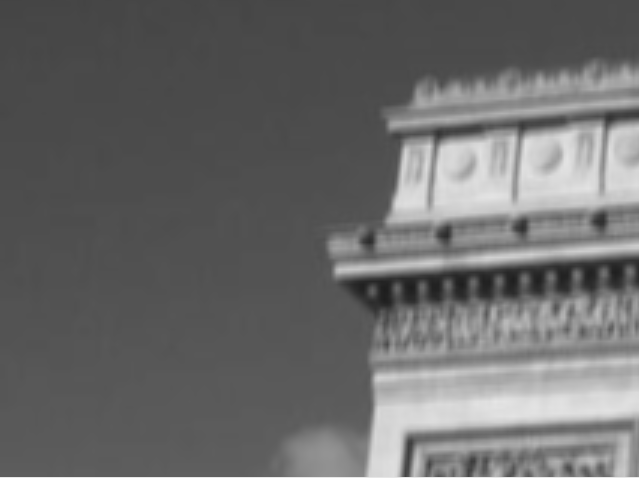
\includegraphics[width=0.9\linewidth]{ressource/detail_flou2.png}
\caption{Input 2}
\label{fig:Flou2}
\end{subfigure}
\begin{subfigure}{0.24\textwidth}
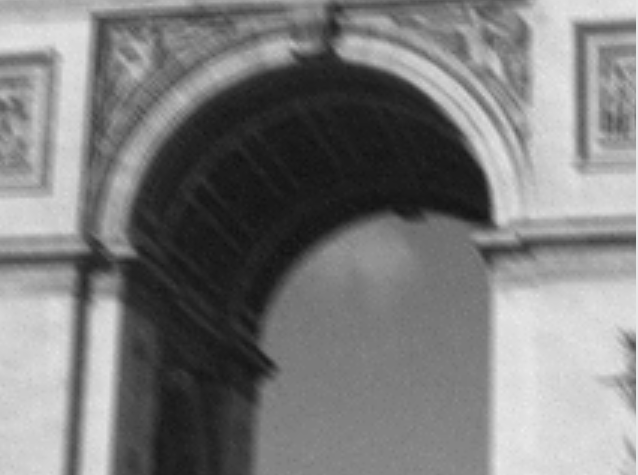
\includegraphics[width=0.9\linewidth]{ressource/detail_flou3.png}
\caption{Input 3}
\label{fig:Flou3}
\end{subfigure}
\begin{subfigure}{0.24\textwidth}
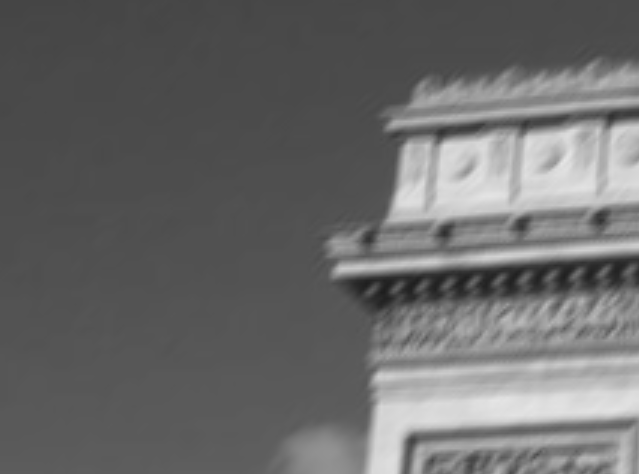
\includegraphics[width=0.9\linewidth]{ressource/detail_flou4.png}
\caption{Input 4}
\label{fig:Flou4}
\end{subfigure}
\begin{subfigure}{0.32\textwidth}
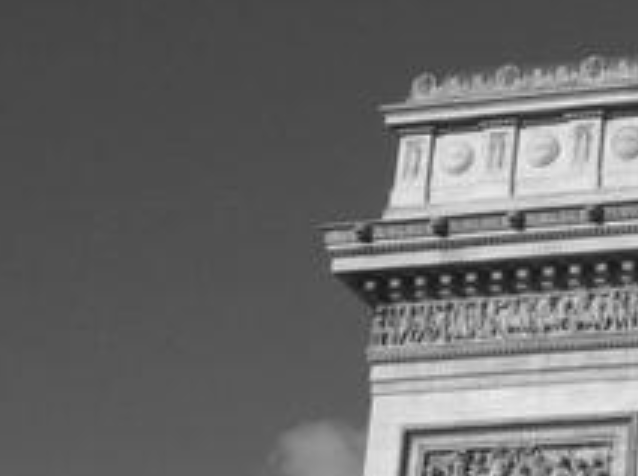
\includegraphics[width=0.9\linewidth]{ressource/detail_orig.png}
\caption{Original sans flou}
\label{fig:Original}
\end{subfigure}
\begin{subfigure}{0.32\textwidth}
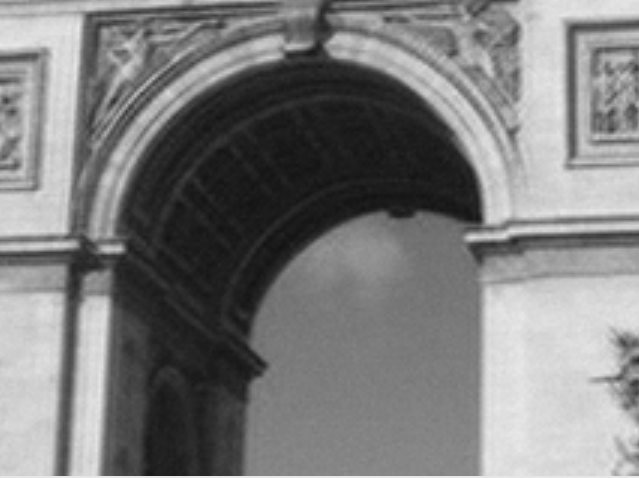
\includegraphics[width=0.9\linewidth]{ressource/detail_result.png}
\caption{Résultat}
\label{fig:Resultat}
\end{subfigure}
\begin{subfigure}{0.32\textwidth}
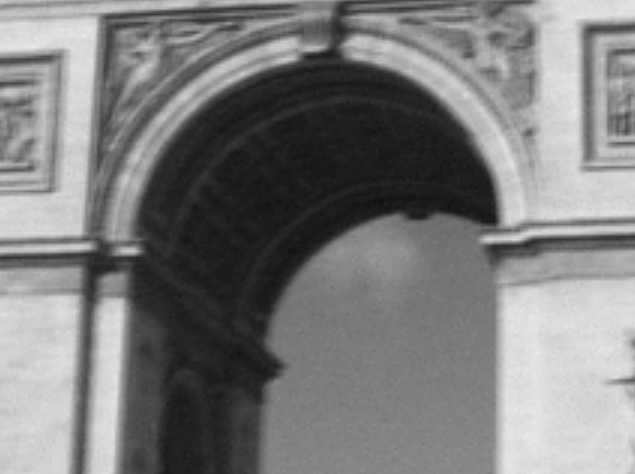
\includegraphics[width=0.9\linewidth]{ressource/detail_flou1.png} 
\caption{Meilleur input}
\label{fig:Bestflou}
\end{subfigure}

\caption{Résultat de l'algorithme pour 4 images recalées}
\label{fig:arctriomphe}
\end{figure}

\paragraph{}
Nous avons ajouté du bruit gaussien uniforme sur les images pour vérifier la robustesse de la méthode
et comme annoncé par l'article cela ne dégrade pas le résultat. On observe même comme attendu un effet
de débruitage plus ou moins efficace selon la quantité d'images utilisées.

\paragraph{}
Nous avons également appliqué l'algorithme aux images anthropologie utlisées par l'article (voir figure~\ref{fig:anthro}
page~\pageref{fig:anthro})


\begin{figure}[h]
 
  \begin{subfigure}{0.32\textwidth}
    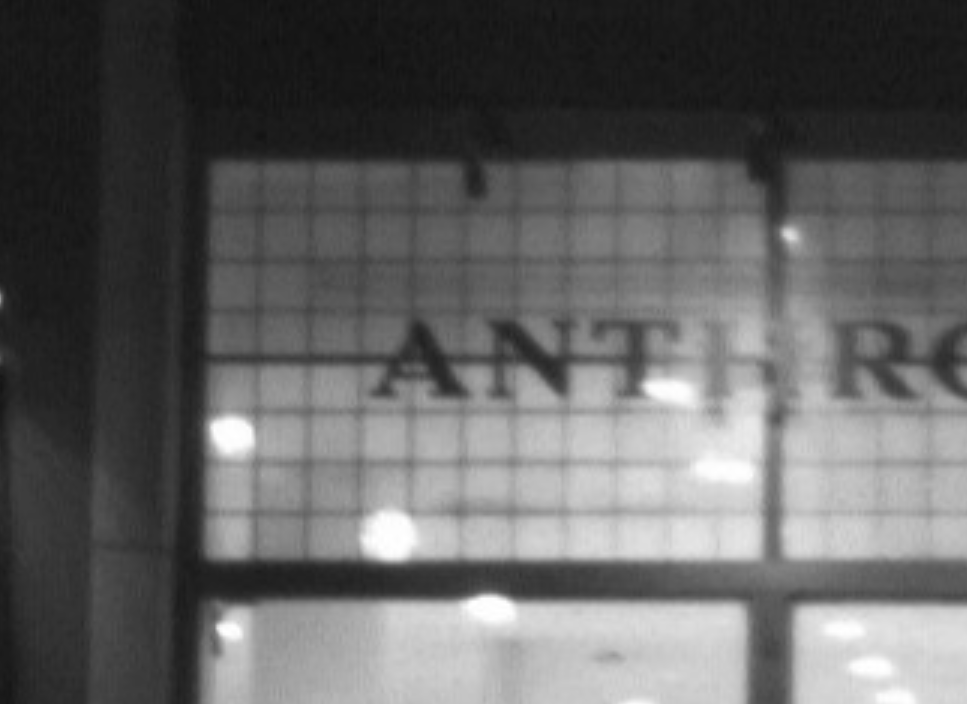
\includegraphics[width=0.9\linewidth]{ressource/detail_anthro1.png} 
    \label{fig:anthro1}
  \end{subfigure}
  \begin{subfigure}{0.32\textwidth}
    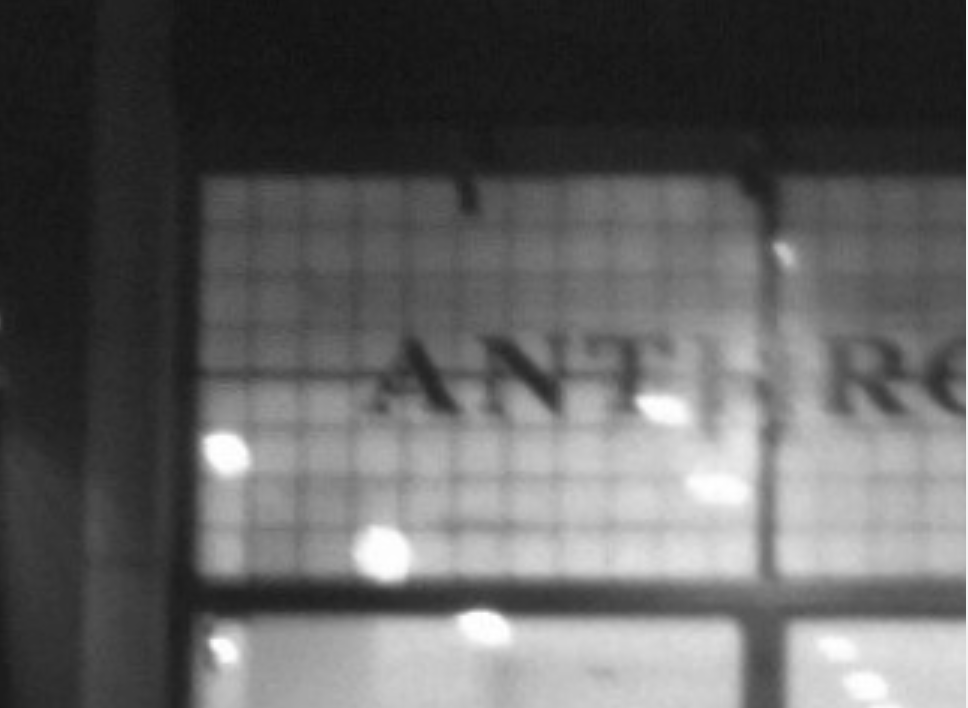
\includegraphics[width=0.9\linewidth]{ressource/detail_anthro3.png} 
    \label{fig:anthro3}
  \end{subfigure}
  \begin{subfigure}{0.32\textwidth}
    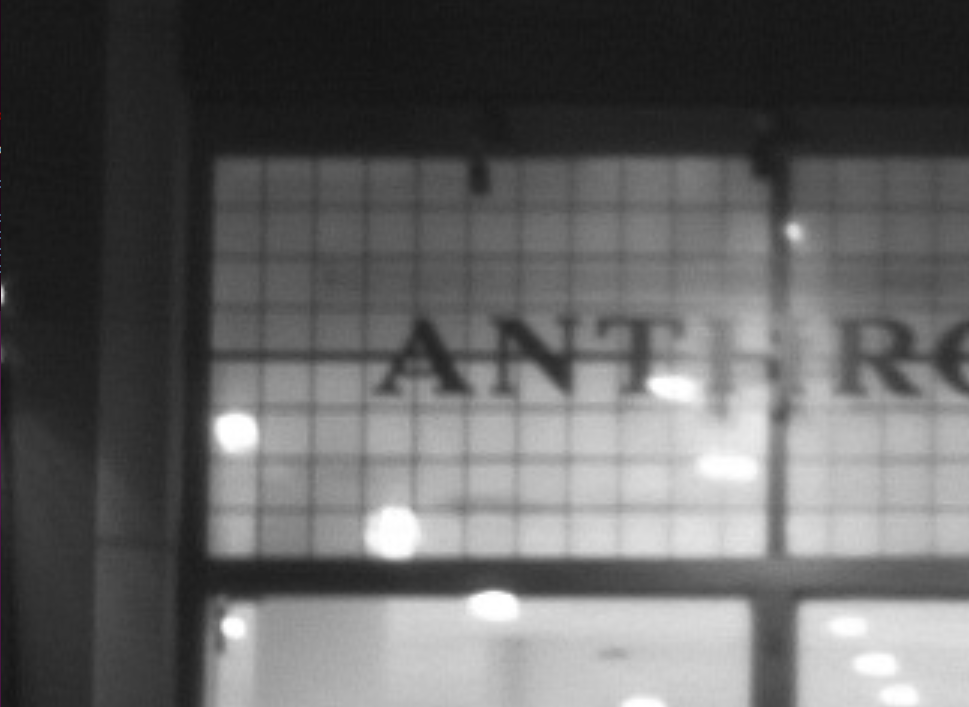
\includegraphics[width=0.9\linewidth]{ressource/detail_anthro_res.png} 
    \label{fig:anthro_result}
  \end{subfigure}
  \begin{subfigure}{0.32\textwidth}
    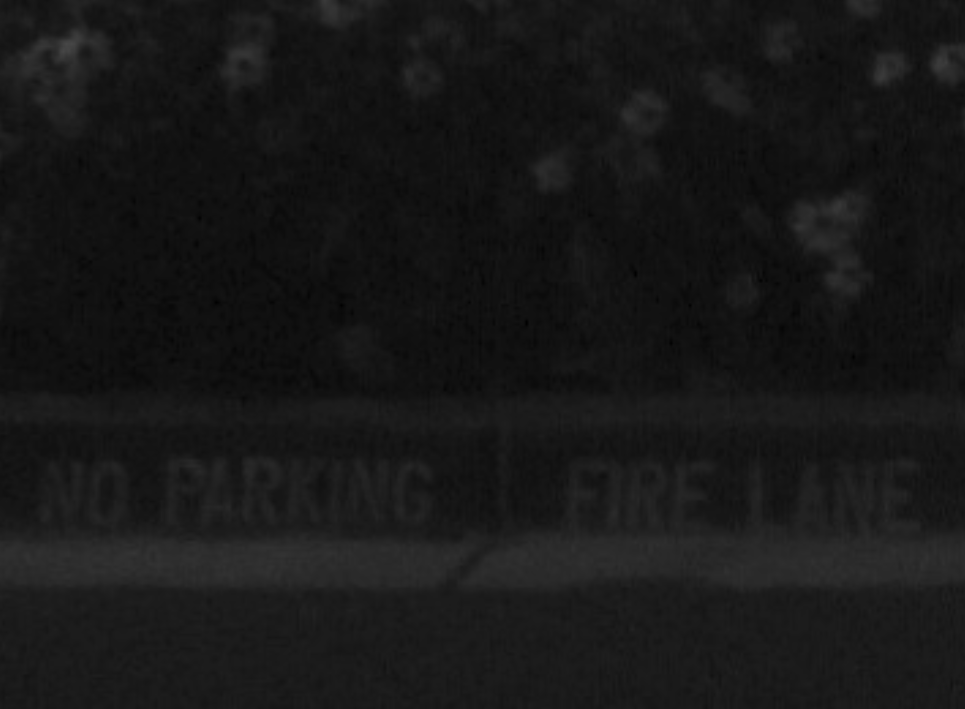
\includegraphics[width=0.9\linewidth]{ressource/detail_fire1.png} 
    \caption{Input 1}
    \label{fig:fire1}
  \end{subfigure}
  \begin{subfigure}{0.32\textwidth}
    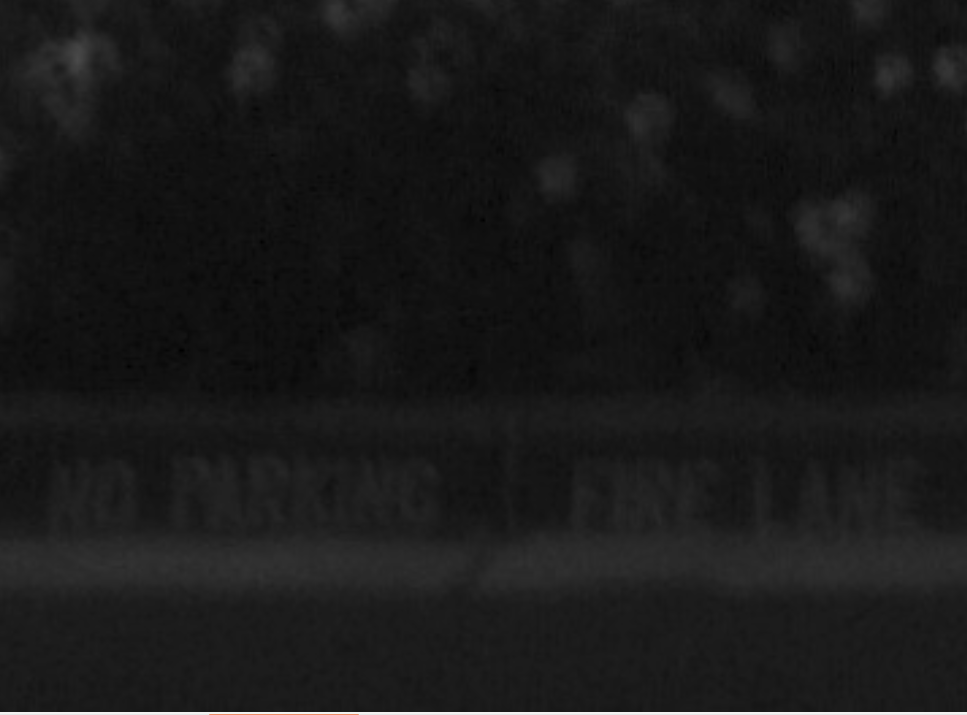
\includegraphics[width=0.9\linewidth]{ressource/detail_fire3.png} 
    \caption{Input 2}
    \label{fig:fire3}
  \end{subfigure}
  \begin{subfigure}{0.32\textwidth}
    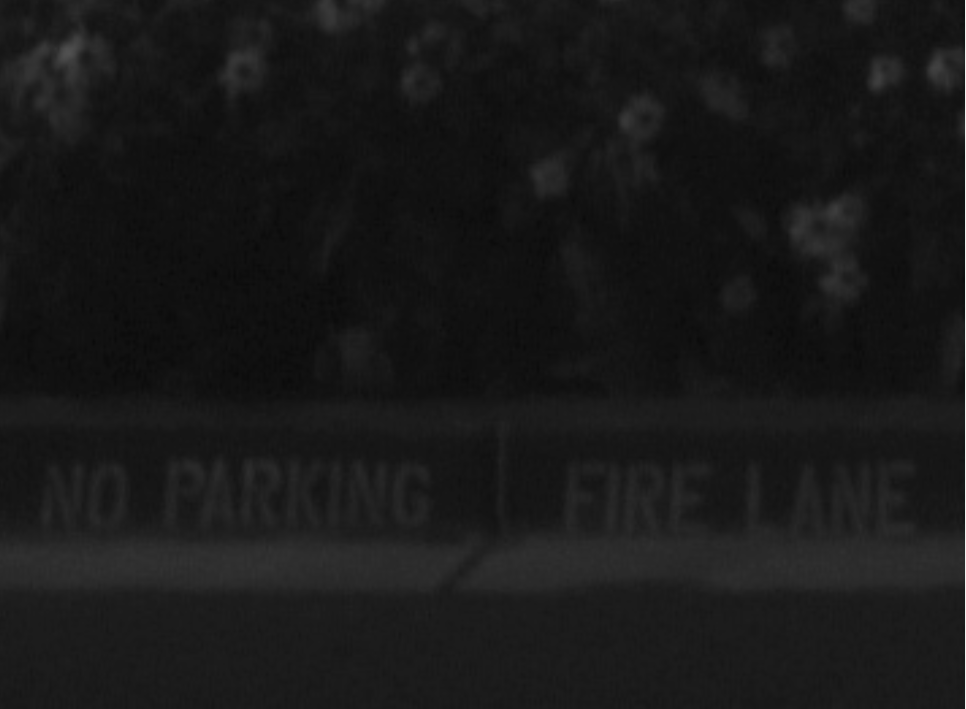
\includegraphics[width=0.9\linewidth]{ressource/detail_fire_res.png} 
    \caption{Resulat}
    \label{fig:fire_result}
  \end{subfigure}
  
  \caption{Résultat de l'algorithme sur les images anthropologies}
\label{fig:anthro}
\end{figure}

\subsection{Influence des paramètres}
\paragraph{}
On observe que le paramètre \(p\) a une grande influence sur la qualité du résultat (voir
figure~\ref{fig:param_p} page~\pageref{fig:param_p}).
Le choix de \(p\) correspond à un compromis entre le biais et la variance du résultat. 
Lorsque \(p\) est proche de 1, on obtient une image peu bruitée mais avec un biais fort : la valeur 
de fréquence choisies tient plus compte des différentes images.
Au contraire avec une grande valeur de \(p\) le biais est plus faible mais la variance augmente,
puisqu'on sélectionne la valeur maximale de la fréquence parmi les différentes images.


\begin{figure}[h]
 
  \begin{subfigure}{0.32\textwidth}
    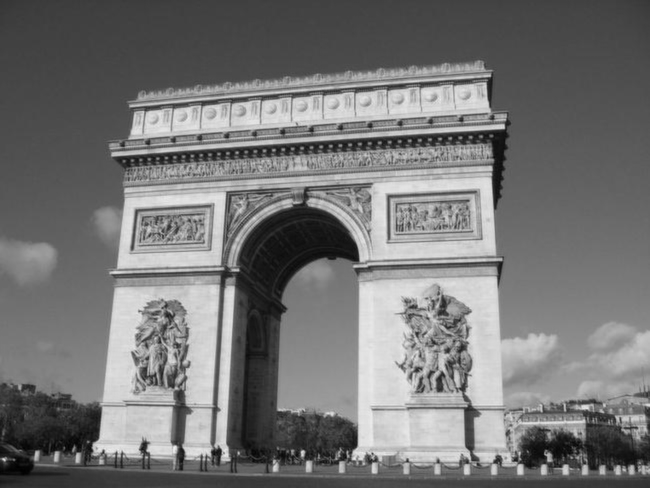
\includegraphics[width=0.99\linewidth]{ressource/flouresultat_p1.png} 
    \caption{\(p=1\)}
    \label{fig:p1}
  \end{subfigure}
  \begin{subfigure}{0.32\textwidth}
    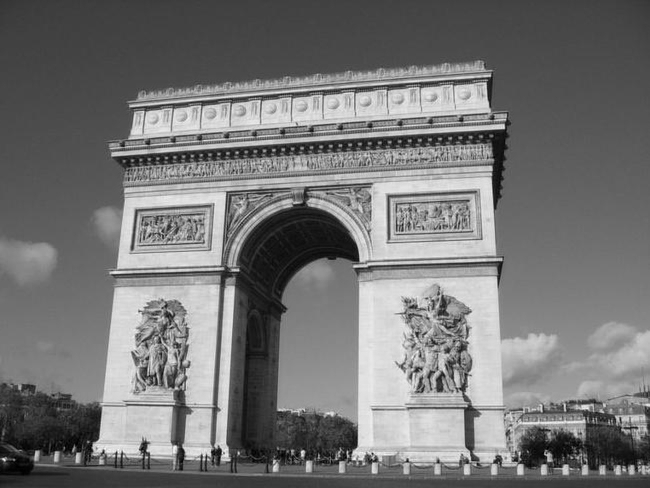
\includegraphics[width=0.99\linewidth]{ressource/flouresultat_p6.png} 
    \caption{\(p=6\)}
    \label{fig:p6}
  \end{subfigure}
  \begin{subfigure}{0.32\textwidth}
    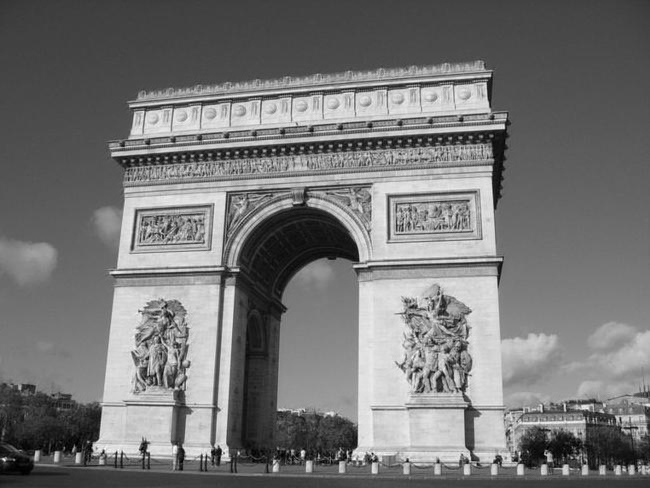
\includegraphics[width=0.99\linewidth]{ressource/flouresultat_p12.png} 
    \caption{\(p=12\)}
    \label{fig:p12}
  \end{subfigure}
  \begin{subfigure}{0.32\textwidth}
    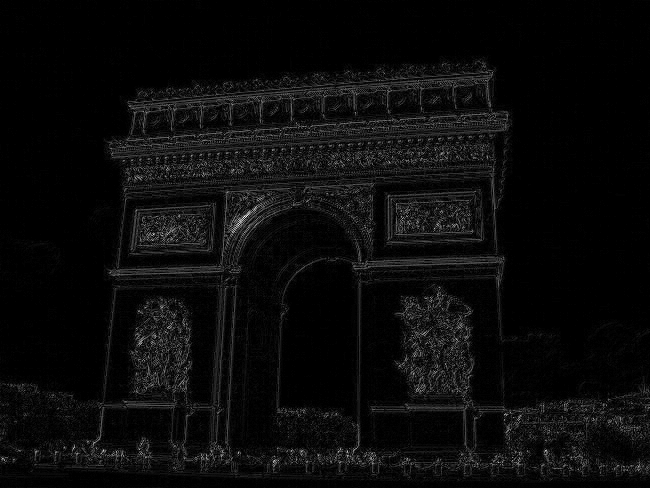
\includegraphics[width=0.99\linewidth]{ressource/diffp1stretch.png} 
    \caption{\(|res_{p=1} - orig|\)}
    \label{fig:diffp1}
  \end{subfigure}
  \begin{subfigure}{0.32\textwidth}
    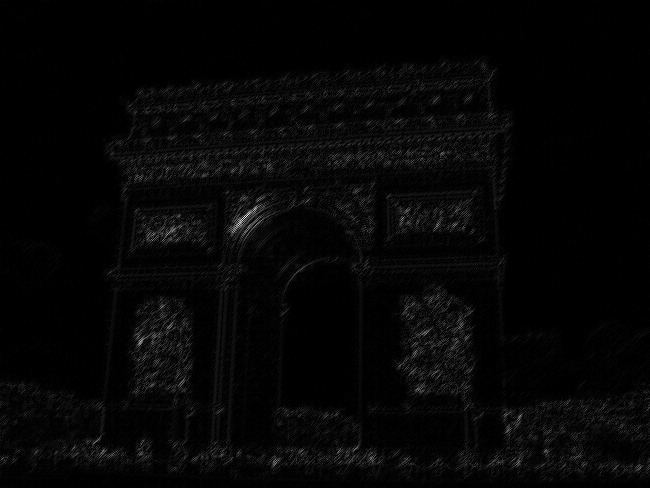
\includegraphics[width=0.99\linewidth]{ressource/diffp6stretch.png} 
    \caption{\(|res_{p=6} - orig|\)}
    \label{fig:diffp6}
  \end{subfigure}
  \begin{subfigure}{0.32\textwidth}
    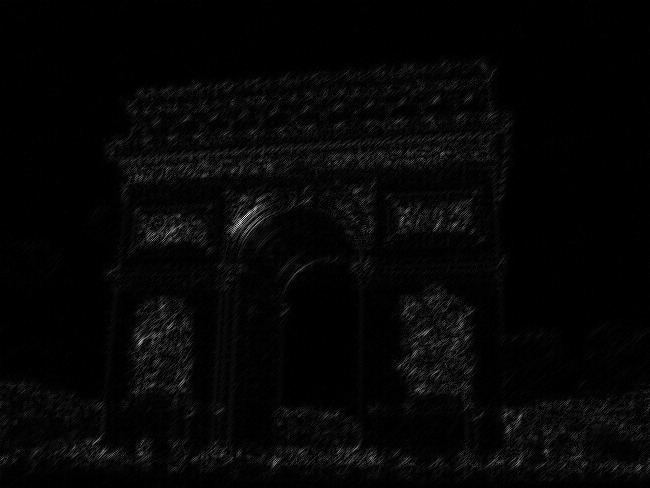
\includegraphics[width=0.99\linewidth]{ressource/diffp12stretch.png} 
    \caption{\(|res_{p=12} - orig|\)}
    \label{fig:diffp12}
  \end{subfigure}
  
  \caption{Influence du paramètre p}
  \label{fig:param_p}
\end{figure}

\subsection{Images non recalées}
\paragraph{}
Mettre une image d'orsa avec inliers

\paragraph{}
Dans la phase de recalage, le nombre d'iteration utilisé joue un rôle très important. Comme on le voit sur 
la figure~\ref{fig:nb_iter} (page~\pageref{fig:nb_iter}), en doublant le nombre d'itérations on obtient un 
recalage plus fin qui permet un meilleur résultat. En effet la moindre erreur de recalage (quelques pixels) 
se traduit par des artefacts dus à des effets de déphasage (Figure~\ref{fig:detail1000iter} page~\pageref{fig:1000iter}). 


\begin{figure}[h]
 
  \begin{subfigure}{0.5\textwidth}
    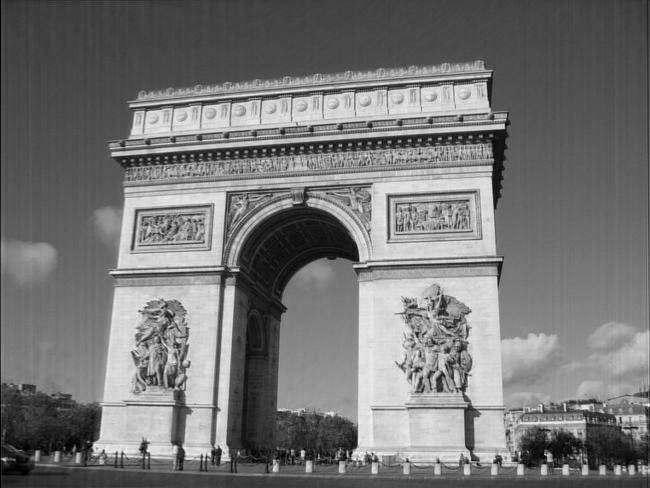
\includegraphics[width=0.99\linewidth]{ressource/arc_result_1000iter.png} 
    \caption{\(n_{iter}=1000\)}
    \label{fig:1000iter}
  \end{subfigure}
  \begin{subfigure}{0.5\textwidth}
    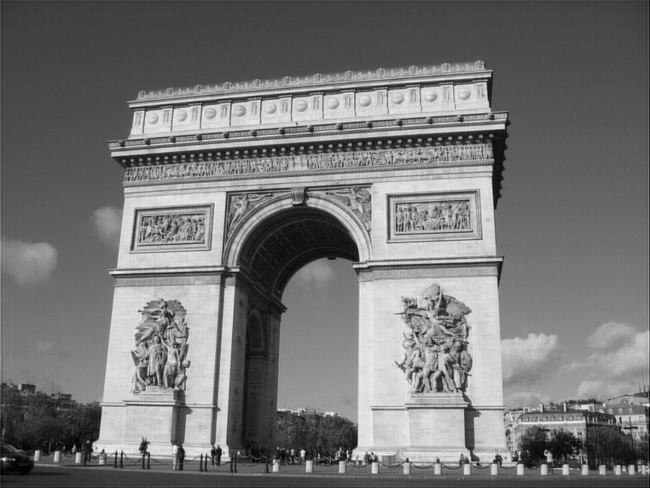
\includegraphics[width=0.99\linewidth]{ressource/arc_result_2000iter.png} 
    \caption{\(n_{iter}=2000\)}
    \label{fig:2000iter}
  \end{subfigure}
  \begin{subfigure}{0.5\textwidth}
    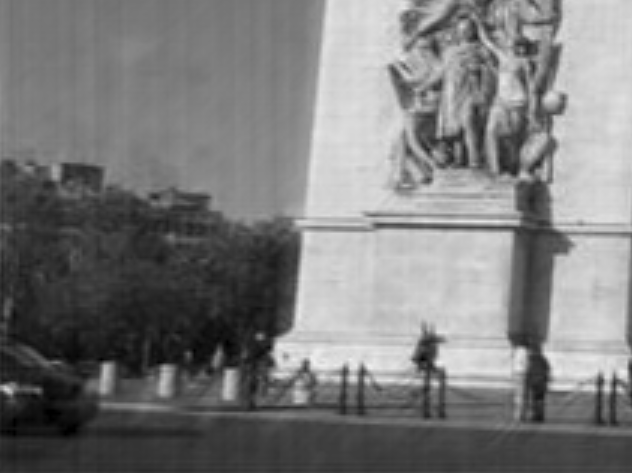
\includegraphics[width=0.99\linewidth]{ressource/detail_1000iter.png} 
    \caption{détail de (a)}
    \label{fig:detail1000iter}
  \end{subfigure}
  \begin{subfigure}{0.5\textwidth}
    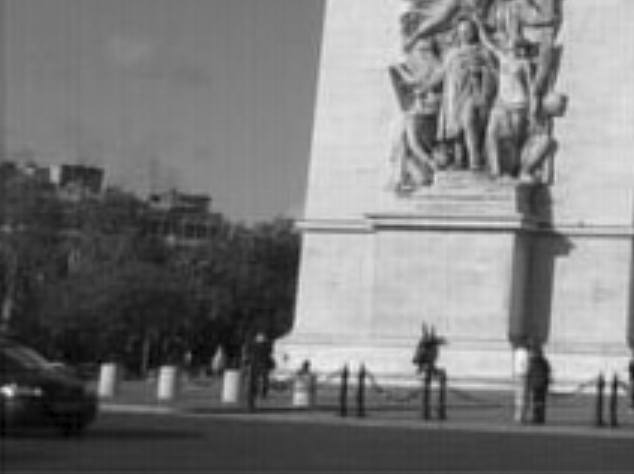
\includegraphics[width=0.99\linewidth]{ressource/detail_2000iter.png} 
    \caption{détail de (b)}
    \label{fig:detail2000iter}
  \end{subfigure}
  
  \caption{Influence du nombre d'itérations}
  \label{fig:nb_iter}
\end{figure}

\section{Analyse et Commentaires}
\paragraph{}
La méthode proposée par l'article donne de bons résultats dans le cas d'images bien recalées. Elle est très 
robuste au bruit et à des noyaux de flous relativement grands (jusqu'à 5 pixels), pas nécessairement en
mouvement rectiligne. Cependant il y a quelques points qui peuvent poser problème.

\subsection{Recalage des images}

\paragraph{}
Le recalage s'avère être le point critique de notre implémentation. 
Une erreur lors du recalage d'une seule des images 
engendre de très gros défauts dans le résultat comme on le voit sur la 
figure~\ref{fig:mauvaisrecalage} (page~\pageref{fig:mauvaisrecalage}).
Ce problème nous a conduit à rejeter les images dont l'estimation d'homographie
s'appuie sur un nombre de points trop faibles. Nous utilisons donc ici le critère : 
image rejetée si \(n_{inliers} < 100\). 
Nous sommes bien sûr conscient qu'un meilleur critère devrait être utilisé. 

\begin{figure}[h]
\centering
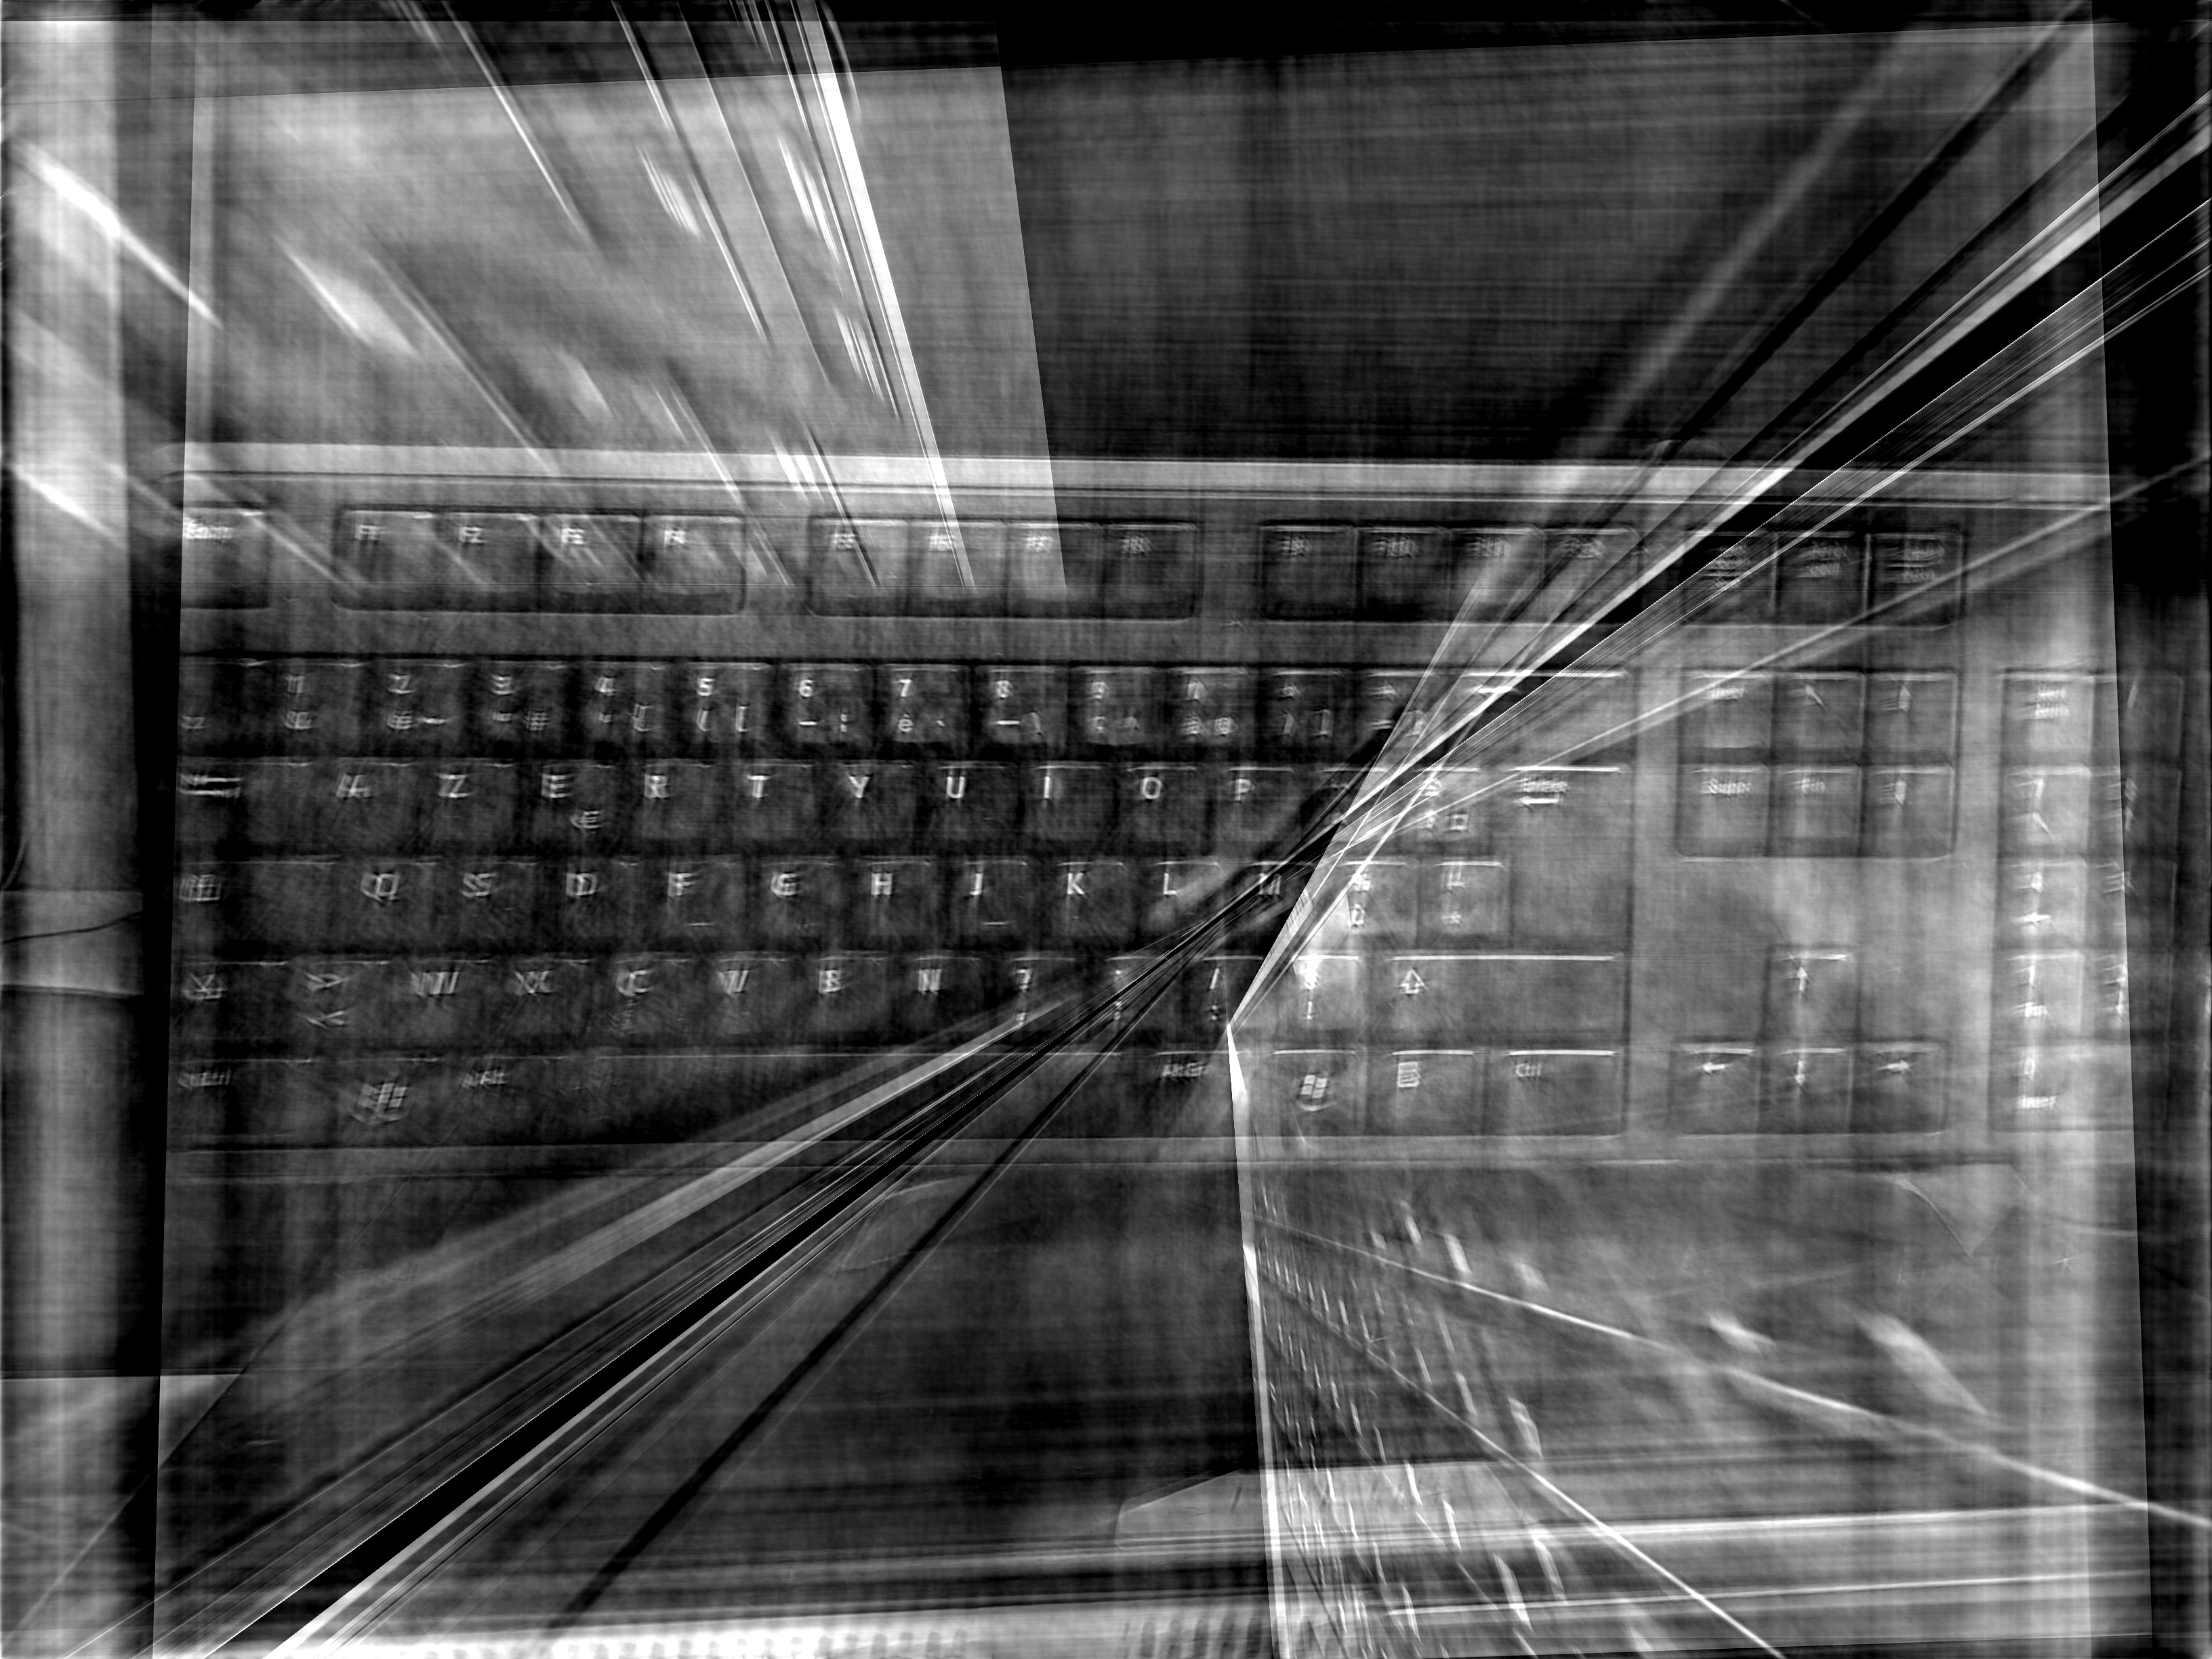
\includegraphics[width=0.5\linewidth]{ressource/keyboardresultat.jpg} 
\caption{Resultat suite à un mauvais recalage}
\label{fig:mauvaisrecalage}
\end{figure}

\paragraph{}
La phase de recalage peut prendre beaucoup de temps, mais est extrêmement importante pour avoir de bons résultats.
Sur nos exemples il est nécessaire d'avoir au moins 2000 iterations dans l'algorithme ORSA pour obtenir un 
recalage satisfaisant et dans certains cas le recalage échoue lorsque les images sont trop floues.
L'article évite cette question en supposant que le recalage est fait immédiatement grâce aux gyroscopes
des smartphones, mais cela peut constituer une limite à l'application de la méthode en temps réel dans 
d'autres appareils. Et effectivement si on se restreint à ce cas d'application on a une méthode rapide et efficace.

\subsection{Flou non homogène : mouvement rotatif}
\paragraph{}
Une limite intrinsèque à cette méthode est l'hypothèse que le flou peut être modélisé comme une convolution
par un noyau. C'est le cas pour les mouvement de translation et de certaines rotations mais ce n'est plus possible 
lorsque l'appareil subit une rotation autour de son axe optique. La PSF dépend alors de la position du pixel dans l'image, 
ce qui ne peut pas être modélisé par une convolution avec un noyau.
\paragraph{}
Ce cas de figure peut pourtant se produire en situation réelle comme nous l'avons constaté 
(voir Figure~\ref{fig:rotation}, page~\pageref{fig:rotation})
Le résultat est très bon au centre de l'image mais se dégrade vers les bords. Une solution envisageable pourrait être
d'appliquer l'algorithme localement sur des portions de l'image suffisamment petites pour que 
l'hypothèse de convolution par un noyau de flou soit valable.

\begin{figure}[h]

\begin{subfigure}{0.32\textwidth}
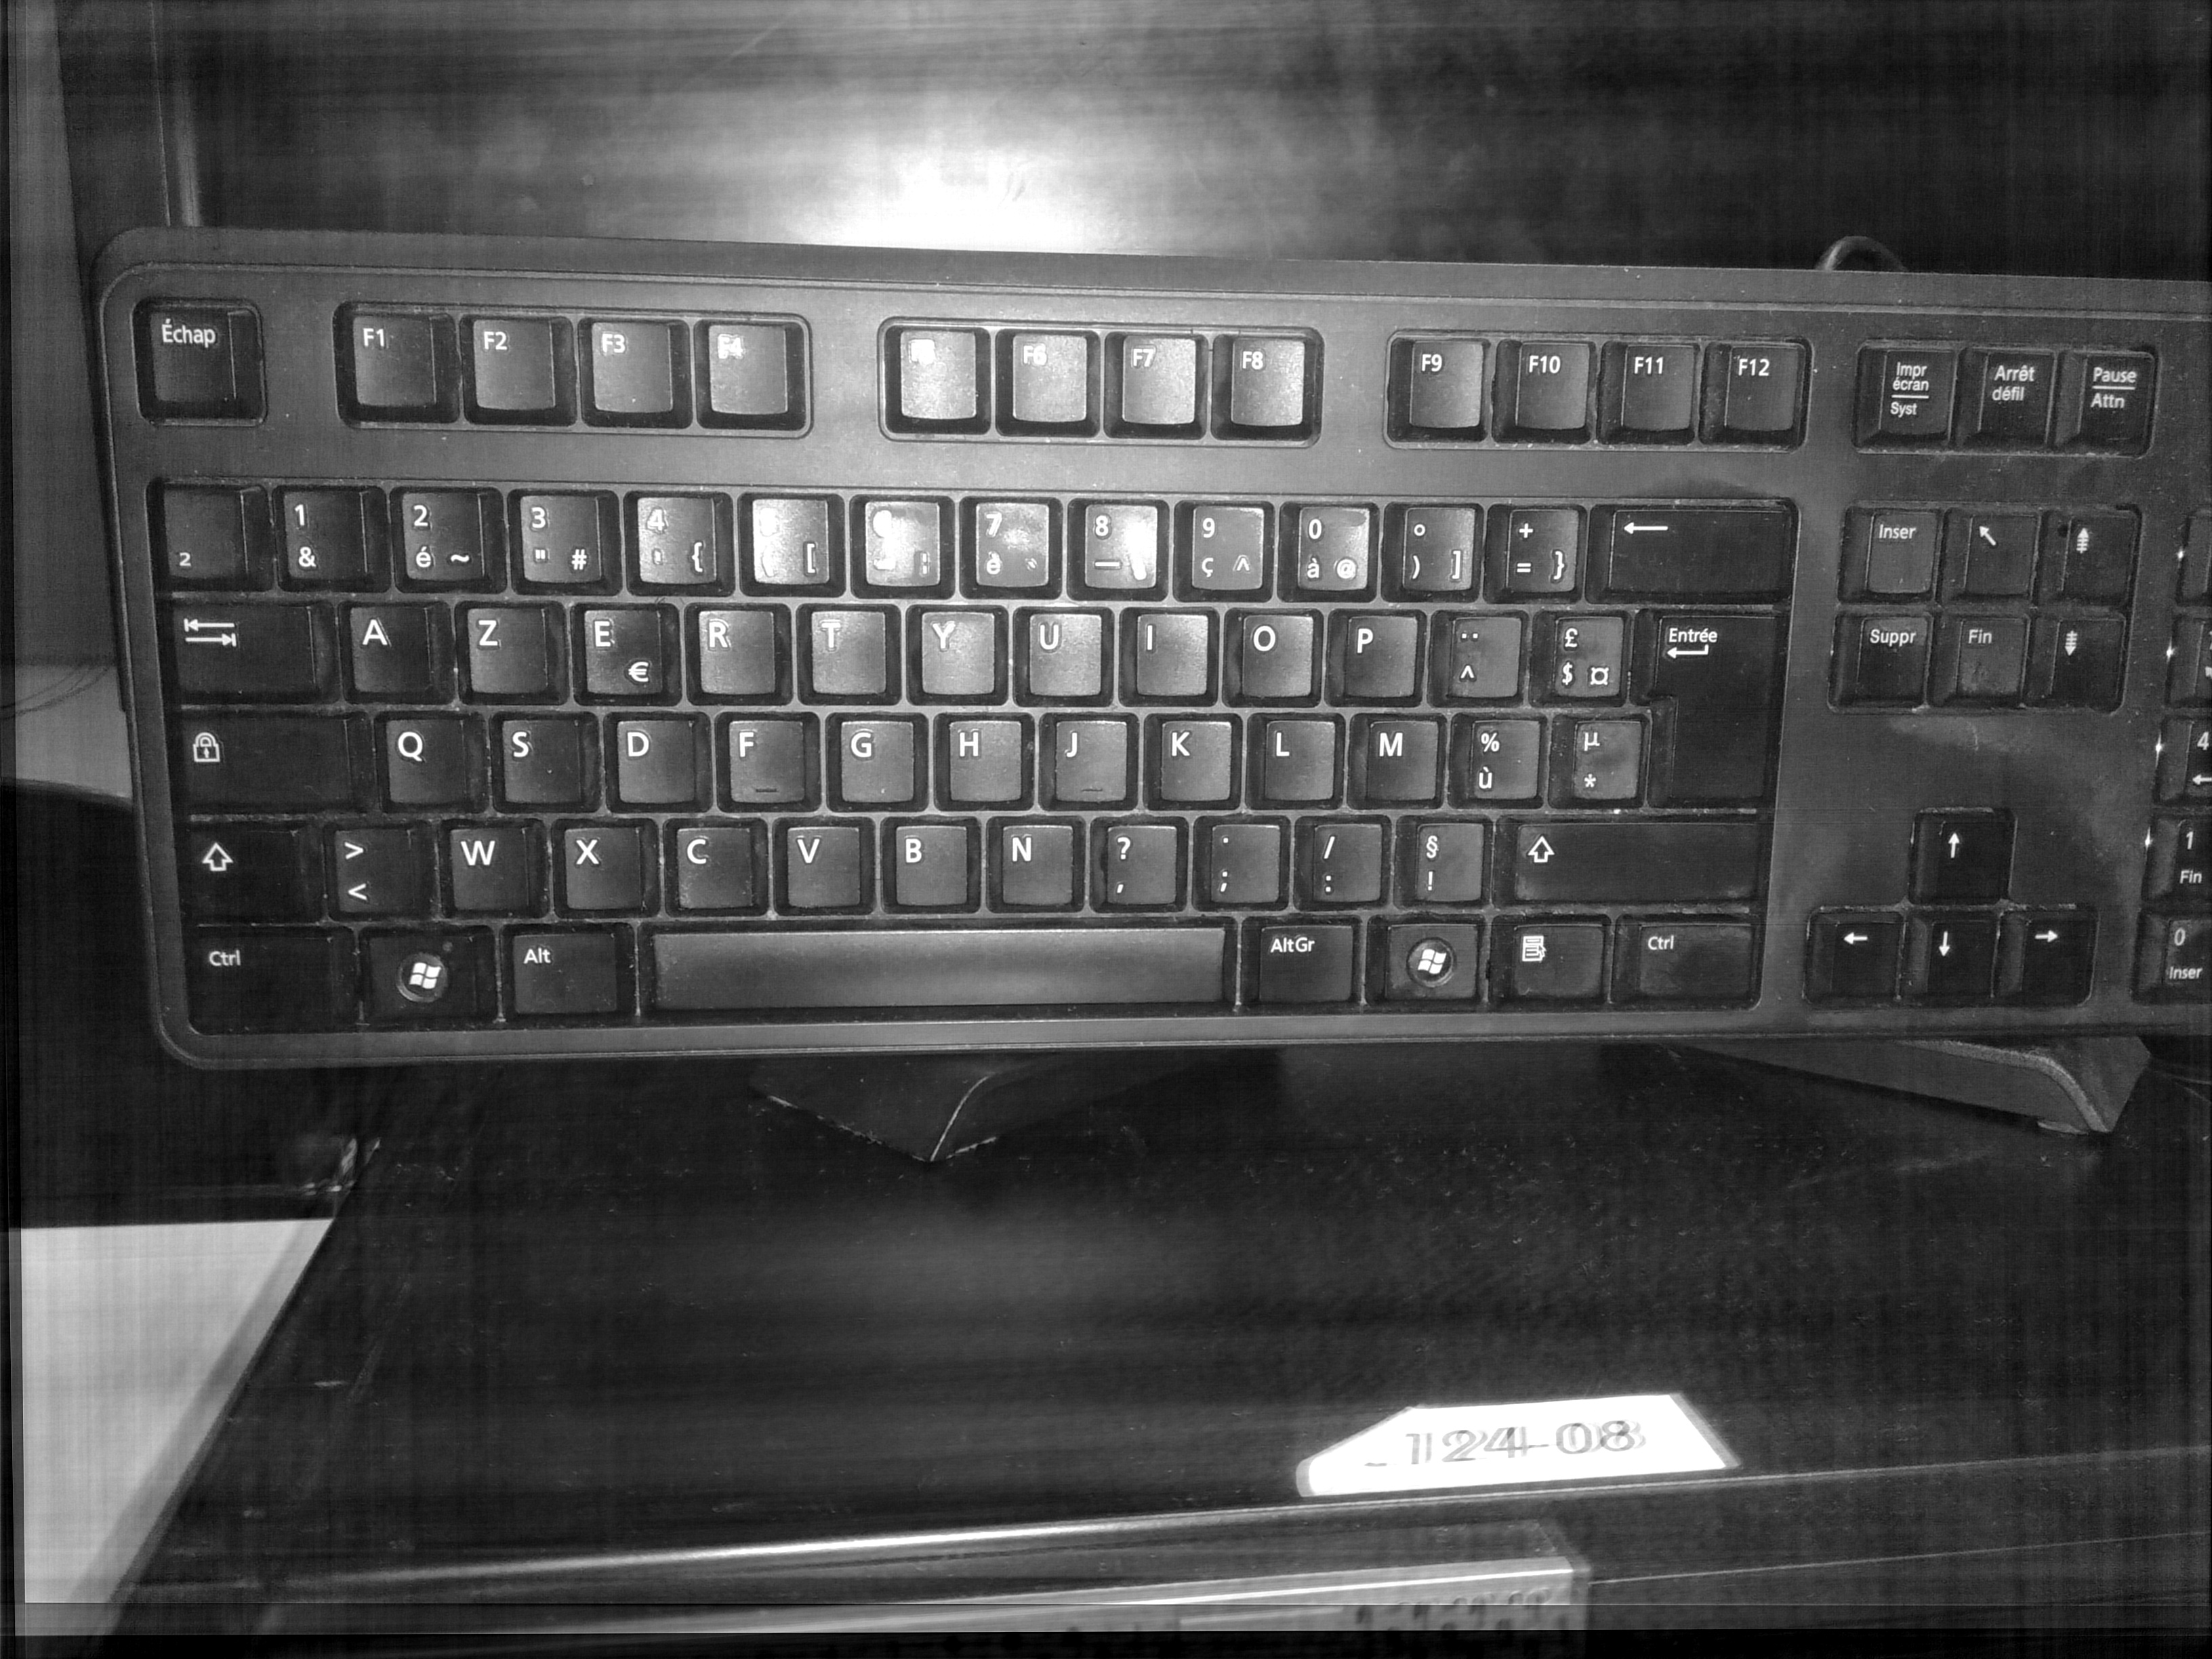
\includegraphics[width=0.9\linewidth]{ressource/flou_rot_10kit.jpg} 
\caption{Resultat}
\label{fig:flourot}
\end{subfigure}
\begin{subfigure}{0.32\textwidth}
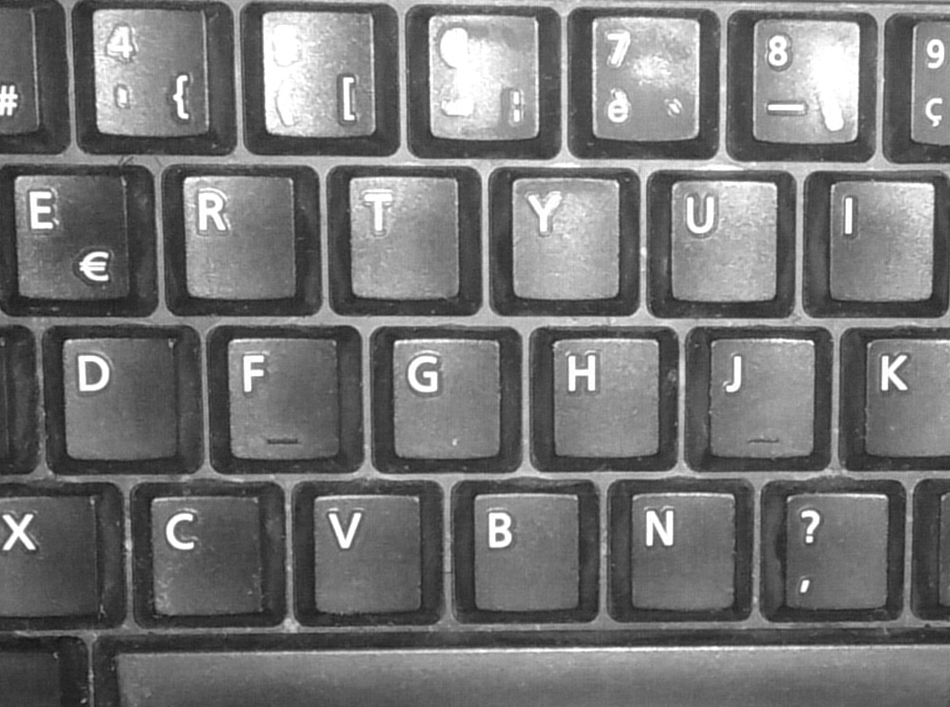
\includegraphics[width=0.9\linewidth]{ressource/flou_rot_centre.png} 
\caption{Centre de l'image}
\label{fig:flouRotCenter}
\end{subfigure}
\begin{subfigure}{0.32\textwidth}
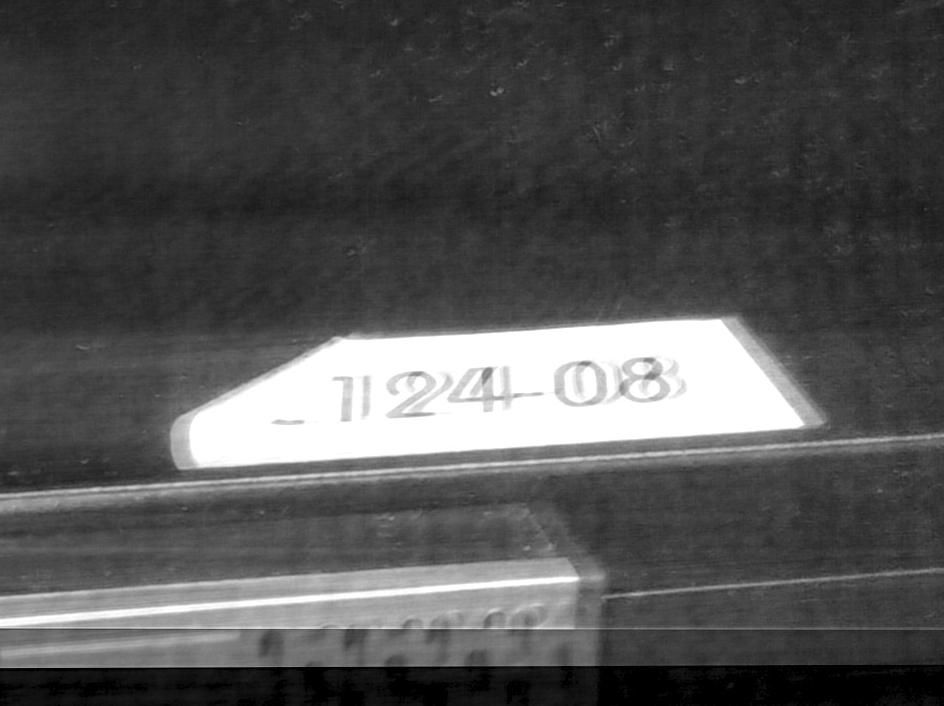
\includegraphics[width=0.9\linewidth]{ressource/flou_rot_bottom.png} 
\caption{Bas de l'image}
\label{fig:flouRotBottom}
\end{subfigure}


\caption{Resultat suite à un flou de rotation}
\label{fig:rotation}
\end{figure}

\end{document}          
